\documentclass[12pt,a4paper]{article}
\usepackage[utf8]{inputenc}
\usepackage[ngerman]{babel}
\usepackage[left=2.5cm,right=2.5cm,top=3cm,bottom=2cm]{geometry}
\author{Pauline Speckmann}
\usepackage{graphicx}
\usepackage{booktabs}
\usepackage{adjustbox}

\usepackage{fancyhdr}
\pagestyle{fancy}
\fancyhf{}
\fancyhead[l]{Digitalisierung Vorlesung 6 $-$ Zusammenfassung von Pauline Speckmann}
\fancyhead[r]{\thepage}


\begin{document}

\setcounter{section}{5}
\section{Digitale Geschäftsmodelle}


\vspace*{1cm}
\subsection{Digitale Güter und Märkte} %%%%%%%%%%%%%%%%%%%%%%%%%%%%%%%%%%%%%%%%%%%%%%%%%%%%%%%%%%%%%%%%%%%%%%%%%%%%%%%%%%%%%%%%%%%%%%%
\begin{itemize}
   \item \textbf{Digitales Gut:}
         \begin{itemize}
            \item Liegen in immaterieller Form vor
            \item Sind vollständig als digitale Repräsentation in Binärform gespeichert
            \item Können ohne Bindung an Trägermedium entwickelt, vertrieben oder angewendet werden (z.B. via Internet)
         \end{itemize}

   \item \textbf{Digitalisierungsgrade von Gütern:}
   \item[] 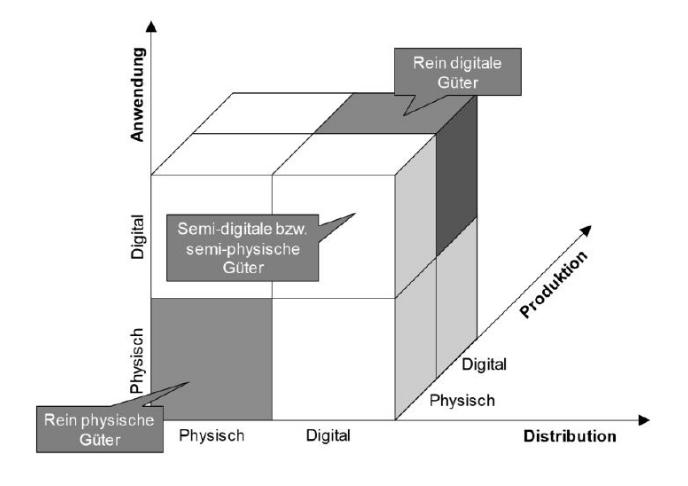
\includegraphics[scale=0.35]{wuerfel.png}
   
   \item \textbf{Eigenschaften digitaler Güter:}
         \begin{itemize}
            \item Wahrnehmungsunterschiede / Interaktivität\\
                  Digitale Güter können nur über zwei Sinne (Sehen und Hören) wahrgenommen werden.
                  Digitale Güter sind interaktiv vom Benutzer bedien- und steuerbar.
            \item Skaleneffekte\\
                  Keine Kostenvorteile entstehen bei durch sinkende Kosten pro hergestelltem Produkt.
            \item Kopierbarkeit / Verteilbarkeit\\
                  Digitale Güter werden bei Weitergabe vermehrt, nicht aufgeteilt.
            \item Veränderbarkeit / Editierbarkeit / Reprogrammierbarkeit\\
                  Digitale Güter können ohne großen Aufwand in Produktvarianten überführt und angeboten werden.
            \item Abnutzbarkeit\\
                  Digitale Güter unterliegen keinerlei Abnutzung; die Unterscheidung zwischen neuem und altem Gut entfällt.
         \end{itemize}

   \item \begin{minipage}[t]{0.43\textwidth}
            \textbf{Modularität} \\
            Möglichkeit der Zerlegung komplexer (Wertschöpfungs-) Systeme in separate Subsysteme, die für sich alleine funktionieren.
         \end{minipage} \begin{minipage}[t]{0.05\textwidth}
            \ \\
         \end{minipage} \begin{minipage}[t]{0.43\textwidth}
            \textbf{Granularität} \\
            Möglichkeit der Zerlegung digitaler Objekte bis in kleinste Elemente und Operationen.
         \end{minipage}

   \item \textbf{Eigenschaften digitaler Märkte:}
         \begin{itemize}
            \item Unendliche Informationsökonomie
                  \begin{itemize}
                     \item Jede Information kann in Form von Bits digitalisiert werden.
                     \item Menschen sind bereit, für Informationen zu zahlen. 
                     \item Der Preis von Informationsgütern richtet sich nach dem Verbraucherwert, nicht nach den Produktionskosten.
                     \item Beispiele von Informationen: Bücher, Datenbanken, Filme etc
                  \end{itemize}
            \item Skaleneffekte\\
                  Entwicklung und Vertrieb digitaler Güter verursachen hohe fixe, aber nur sehr geringe variable Kosten, wodurch sich extreme Skaleneffekte ergeben.
            \item Netzwerkeffekte\\
%                  \vspace*{-0.3cm}
                  \begin{minipage}[t]{0.6\textwidth}\vspace*{-0.3cm}
                     Der Nutzen aus einem Produkt für einen Konsumenten verändert sich, wenn sich die Anzahl gleicher oder komplementärer Parteien im Markt verändert.
                  \end{minipage} \begin{minipage}[t]{0.05\textwidth}\vspace*{-0.3cm}
                     $\ $\\
                  \end{minipage} \begin{minipage}[t]{0.3\textwidth}\vspace*{-0.3cm}
                     \includegraphics[scale=0.25]{network.png}
                  \end{minipage}
            \item Lock-In Effekte\\
                  Starke Kundenbindung an Produkte/Dienstleistungen durch hohe Wechselkosten oder Wechselbarrieren.
            \item Versionierung\\
                  Informationsprodukt in verschiedenen Versionen für verschiedene Marktsegmente anbieten
         \end{itemize}
\end{itemize}


\vspace{1cm}
\subsection{Geschäftsmodelle} %%%%%%%%%%%%%%%%%%%%%%%%%%%%%%%%%%%%%%%%%%%%%%%%%%%%%%%%%%%%%%%%%%%%%%%%%%%%%%%%%%%%%%%%%%%%%%%%%%%%%%%%
\begin{itemize}
   \item \textbf{Definition von Geschäftsmodellen:}
   \item[] 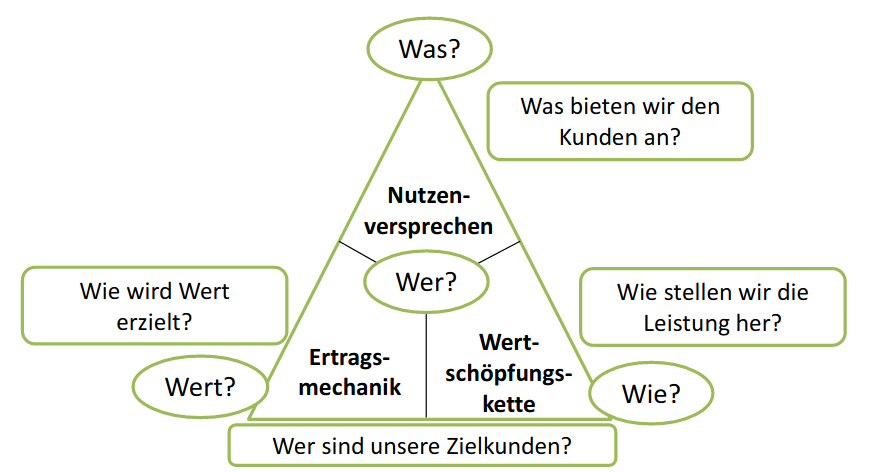
\includegraphics[scale=0.4]{wfragen.png}
   
   \newpage
   \item \textbf{Geschäftsmodelltypen:}
         \begin{itemize}
            \item \textbf{Produkt-Geschäftsmodell}
                  \begin{itemize}
                     \item standardisierte Produkte und Dienstleistungen
                     \item breite Kundenbasis
                     \item tiefe Transaktionskosten
                     \item Differenzierung durch Preis oder Leistung
                     \item Beispiel: Autos
                  \end{itemize}
            \item \textbf{Plattform-Geschäftsmodell}
                  \begin{itemize}
                     \item gemeinsame, integrative Architektur 
                     \item große Bandbreite oder Tiefe oft digitaler Angebote
                     \item Netzwerkeffekte für die Nutzer der Plattform
                     \item Differenzierung über Nutzerzahlen
                     \item Beispiel: soziale Netzwerke
                  \end{itemize}
            \item \textbf{Projekt-Geschäftsmodell}
                  \begin{itemize}
                     \item kundenindividuelle Produkte und Dienstleistungen
                     \item einmalige Leistungsvereinbarungen
                     \item Differenzierung durch Flexibilität
                     \item hoher Serviceanteil
                     \item Beispiel: Aufzug bauen
                  \end{itemize}
            \item \textbf{Lösungs-Geschäftsmodell}
                  \begin{itemize}
                     \item Kombination kundenindividueller Angebote
                     \item integrierte End-to-End Leistungen
                     \item langfristige Verträge
                     \item gegenseitige Abhängigkeit zwischen Anbieter und Abnehmer
                     \item Beispiel: Logistik
                  \end{itemize}
         \end{itemize}

   \item \textbf{Eigenschaften digitaler Geschäftsmodelle:}
   \item[] 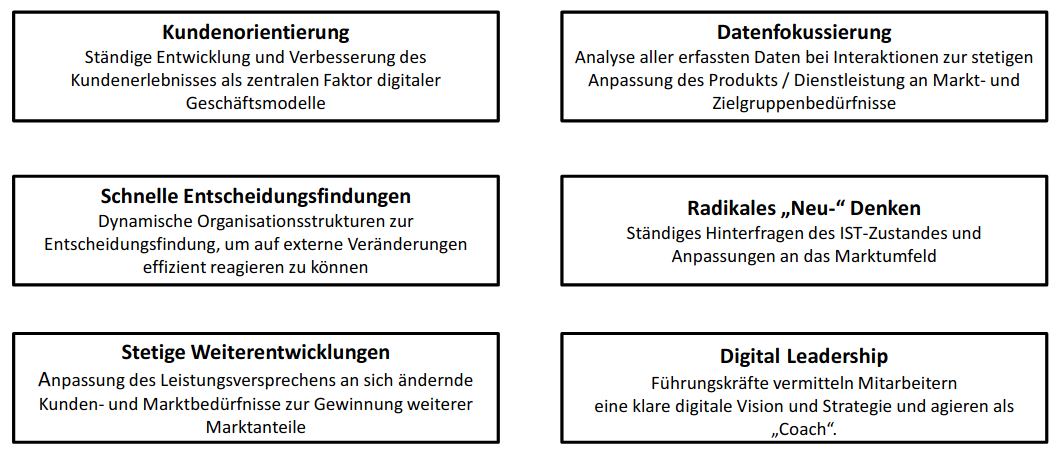
\includegraphics[scale=0.4]{edg.png}
   
   
   \newpage
   \item \textbf{Potenziale durch internen und externen Digitalisierungsfokus}
   \item[] 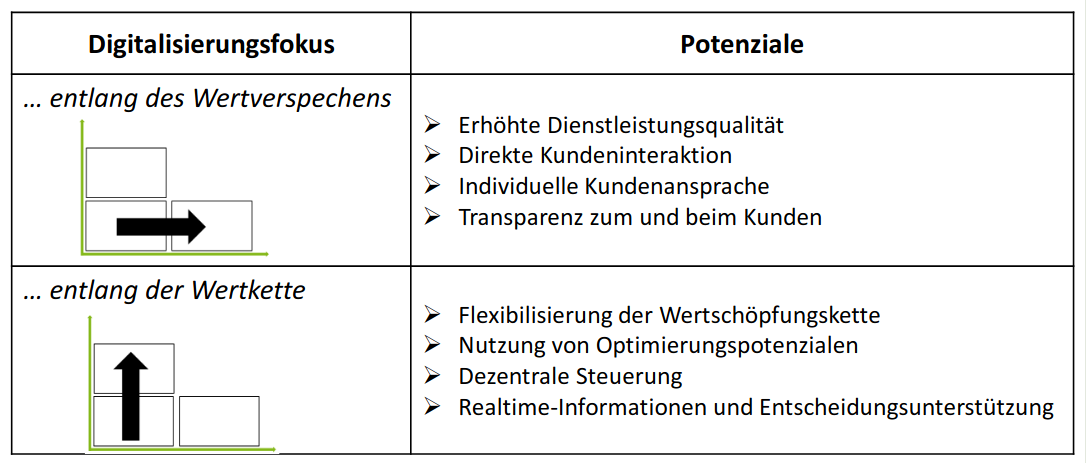
\includegraphics[scale=0.45]{potdig.png}
   
   \item \textbf{Häufige Geschäftsmodellmuster digitaler Unternehmen}
			\begin{itemize}
				\item \textbf{Freemium:}\\
						Kostenlose Basisversion und Premiumversion, oft als Abo-Modell (Dropbox)
				\item \textbf{Abonnement / Subscription:}\\
				      Nutzung der Leistung in regelmäßigen Abständen, Vertragliche Vereinbarung zwischen Kunde und Unternehmen, Zahlung in regelmäßigen Zeitabständen (Netflix)
				\item \textbf{Add-On:}\\
						Nutzen eines Services oder Produkts zu einem möglichst geringen Kaufpreis anbieten. Durch gebührenpflichtige Zusätze kann das Produkt beliebig erweitert werden (SAP)
				\item \textbf{Lock-In:}\\
						Kunden werden an ein Produkt gebunden, indem die Kosten für einen Ausstieg oder Wechsel gesteigert werden (AmazonPrime)
				\item \textbf{Rent instead of buy:}\\
						Unternehmen verkauft das Produkt nicht, sondern gewährt Kunden gegen einen kleineren Betrag zeitlich limitierte Nutzungsrechte (E-Scooter leihen)
				\item \textbf{Plattform / Mehrseitige Märkte:}\\
						Unterscheidbare Nutzergruppen, werden auf der Plattform eines Dritten zusammengeführt (Google)
			\end{itemize}
\end{itemize}


\vspace{1cm}
\subsection{Modellierung von Geschäftsmodellen} %%%%%%%%%%%%%%%%%%%%%%%%%%%%%%%%%%%%%%%%%%%%%%%%%%%%%%%%%%%%%%%%%%%%%%%%%%%%%%%%%%%%%%
\begin{itemize}
   \item \textbf{Ziele:}
		   \begin{itemize}
				\item Kernelemente und -logik eines Geschäftsmodells visualisieren
				\item Existierende Geschäftsmodelle besser verstehen
				\item Ideen für neue, innovative Geschäftsmodelle zu generieren
			\end{itemize}
	
	
	\newpage
	\item \textbf{Business Model Canvas (BMC):}
	      \begin{itemize}
				\item Kundennutzen (\emph{Value Proposition}) stellt Kern dar
				\item Leitfragen:
				\item[] 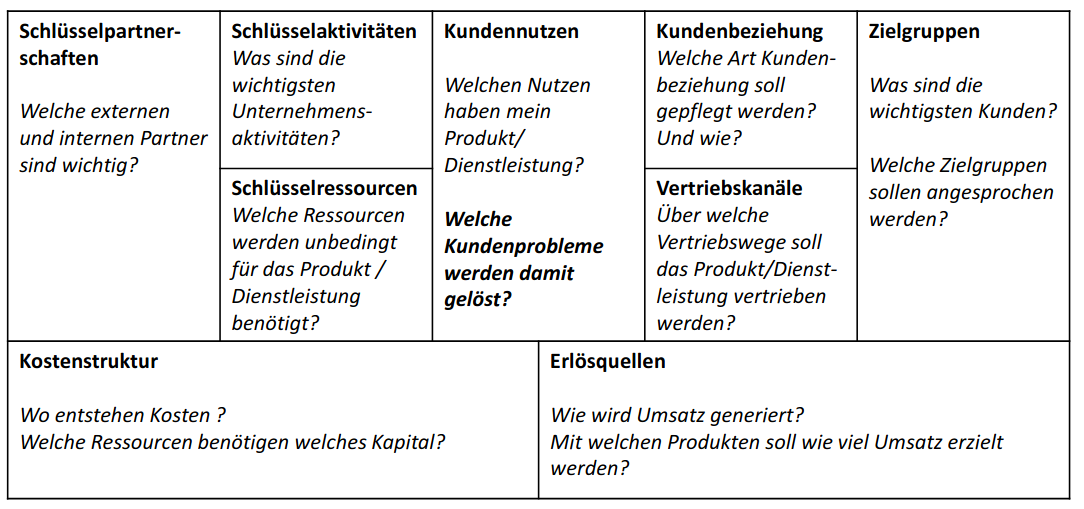
\includegraphics[scale=0.35]{BMC.png}
			\end{itemize}
	
	\item \textbf{e$^3$-Value Modellierung:}
	      \begin{itemize}
				\item Modellierungsobjekte:
				\item[] 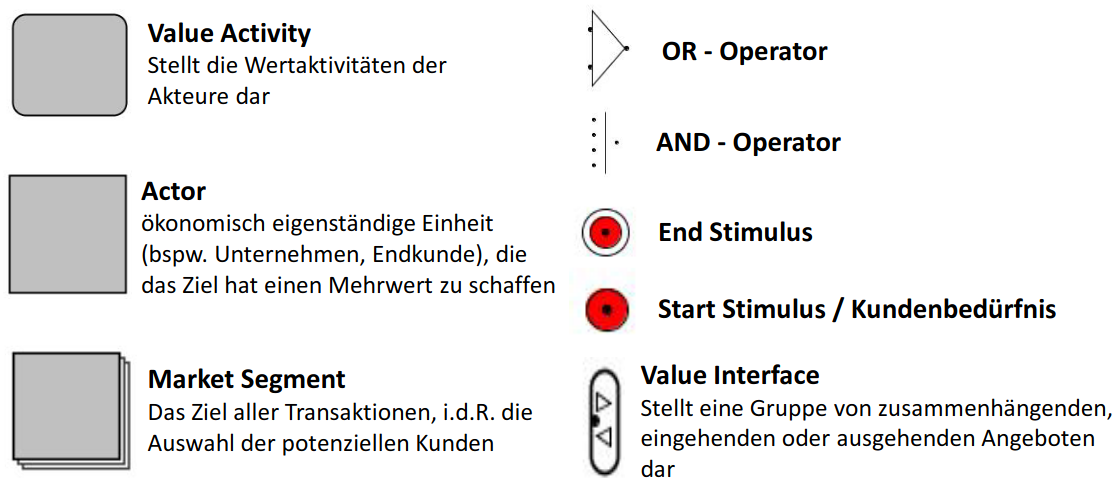
\includegraphics[scale=0.35]{modelldings.png}
				\item Beispiel eines solchen Modells:
				\item[] 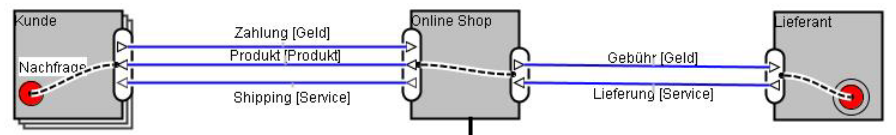
\includegraphics[scale=0.5]{beispiel_e3.png}
			\end{itemize}
	
	\item \textbf{BMC vs. e$^3$-Value:}
	\item[] \adjustbox{max width=0.9\textwidth}{%
			\begin{tabular}{r l l}
			\toprule
			    & \textbf{BMC} & \textbf{e$^3$-Value} \\
			\midrule
			\textbf{Stärken:} & ganzes Geschäftsmodell wird beschrieben & Schnittstellen werden dargestellt \\
			 & deutliche Herausstellung der Value Proposition\footnotemark & Berechnung des Wertflusses \\
			 & & Nutzenanalysen pro Akteur möglich \\
			 & &  \\
			\textbf{ Schwächen:} & keine Darstellung d. Interaktion von Akteuren & Datenbasis muss vorhanden sein \\
			 & fehlender Detaillierungsgrad & Hohe Komplexität bei größeren Netzwerken \\
			 & fehlende Nutzungsbeurteilung & keine Herausstellung der Value Proposition \\
			  & &  \\
			\textbf{Innovationsgrad:} & bei radikalen Innovationen sinnvoll & bei inkrementellen\footnotemark \ Innovationen sinnvoll \\
			\bottomrule
			\end{tabular}}
\end{itemize}

\footnotetext[4]{Nutzenversprechen (englisch value proposition) beschreibt, welchen Nutzen ein Unternehmen seinen Kunden mit einem bestimmten Produkt oder einer bestimmten Dienstleistung verspricht. }

\footnotetext[5]{Bei inkrementeller Innovation werden bekannte Technologien, Produkte, Dienstleistungen, Geschäftsmodelle oder Prozesse weiterentwickelt, bleiben aber im Kern erhalten.}



\vspace{1cm}
\subsection{QUIZFRAGEN} %%%%%%%%%%%%%%%%%%%%%%%%%%%%%%%%%%%%%%%%%%%%%%%%%%%%%%%%%%%%%%%%%%%%%%%%%%%%%%%%%%%%%%%%%%%%%%%%%%%%%%%%%%%%%%
\begin{itemize}
   \item Rein digitale Geschäftsmodelle basieren auf der Sammlung von Informationen und der Verarbeitung dieser.
   \item Digitale Güter lassen sich erschwert vergleichen und es herrscht eine Informationssymmetrie zwischen Preis und Qualität.
   \item Im Gegensatz zu nicht-digitalen Gütern besteht kein Unterschied zwischen dem Original und einer Kopie.
         Eine Duplizierung bei digitalen Gütern ist einfacher als bei nicht-digitalen Gütern.
   \item Die Skaleneffekte digitaler Güter ermöglichen hohe Marktanteile durch die Fixkostendegression.
   \item Anwendungssoftware oder \textit{Cloud-Comuting} Dienstleistungen sind \emph{keine} rein digitalen Güter.
   
   \item Für die \textit{e3-Value}-Methode sind sinnvolle Daten essentiell, um den vollen Nutzen zu generieren.
   \item Die \textit{e3-Value}-Methode benötigt eine hohe Datenintegration um sinnvolle Ergebnisse zu liefern.
   \item Anders als das BMC (\textit{Business Model Canvas}) ist eine umfassende Wirtschaftlichkeitsanalyse bei der \textit{e3-Value}-Methode möglich.
   \item Das BMC (\textit{Business Model Canvas}) sollte in der frühen Innovationsphase angewendet werden, da es einen guten Überblick über das ganzheitliche Geschäftsmodell liefert.
         Es stellt den Kundennutzen sehr deutlich heraus.
   \item Die Modellierung eines Geschäftsmodells kann \emph{nicht} verwendet werden, um Konkurrenten im Markt detailliert zu analyisieren.
   
   \item Auf dem digitalen Markt ist der Lock-in-Effekt ein Mittel der Netzwerkanbieter, um Kunden stärker an sich zu binden.
         Durch starke Skaleneffekte können Monopole entstehen.
   \item Auf elektronischen Märkten können sich $n$ Nachfrager und $m$ Anbieter in einer $n:m$-Beziehung gegenüberstehen.
   \item Die Markttransparenz auf elektronischen Märkten ist als hoch einzustufen.
\end{itemize}
\end{document}






